\documentclass[xcolor=table]{beamer}

\usetheme[secheader,compress]{Madrid} %Primary theme

\usepackage{verbatim}
\usepackage{graphicx}

%% UTM Colors
\definecolor{UTMblue}{rgb}{0.043137, 0.137254, 0.254901}
\definecolor{UTMorange}{rgb}{1.0, 0.509803, 0}

\setbeamercolor{palette primary}{bg=UTMblue,fg=white}
\setbeamercolor{palette secondary}{bg=UTMblue,fg=white}
\setbeamercolor{palette tertiary}{bg=UTMblue,fg=white}
\setbeamercolor{palette quaternary}{bg=UTMblue,fg=white}
\setbeamercolor{structure}{fg=UTMblue} % itemize, enumerate, etc
\setbeamercolor{section in toc}{fg=UTMblue} % TOC sections
\setbeamercolor{title}{fg=UTMorange}

\setbeamercolor{subsection in head/foot}{bg=UTMorange,fg=white}

%%%%%%%%%%% BEGIN MACROS %%%%%%%%%%%%%%%%%%
% frameT: Frame with title
\newcommand{\frameT}[2]{\frame{\frametitle{#1} #2}}

% frameF: Fragile frame with title
\newcommand{\frameF}[2]{
  \begin{frame}[fragile]
    \frametitle{#1}
    #2
  \end{frame}
}

% frameTop: Frame aligned t the top
\newcommand{\frameTop}[2]{\frame[t]{\frametitle{#1} #2}}


\newcommand{\tab}{\hspace{1cm}}

\newcommand{\spaceor}{\hspace{5pt} \textbf{or} \hspace{5pt}}

%%%%%%%%%%% END MACROS %%%%%%%%%%%%%%%%%%%%



\begin{document}

\title{The Deep Journey}

\author{James Blankenship and Andrew Marshall}
\institute{UT-Martin}
\date{\today}

%%%%%%%%%%% BEGIN TITLE %%%%%%%%%%%%%%%%%%
\frame{\titlepage}

 %\section{Outline}
%%%%%%%%%%%% END TITLE  %%%%%%%%%%%%%%%%%%



\section{Introduction}

  
  \section{Background}
  \frameT{Overview}{
    
  Overview of project 
  \bigskip
  \begin{enumerate}
  \item Made in the unreal engine.
    \bigskip
  \item Real time combat in the first person
    \bigskip
  \item Multiple levels in game.
    \bigskip
    \item It is in the fantasy genre
  \end{enumerate}
  }
  \frameT{Overview}{
  \section{Overview cont.}
  
  Overview of Project cont.
  \begin{enumerate}
    \item Each level will focus on a enemy race.
    \bigskip
  \item Enemy types are orcs goblins and humans.
    \bigskip
  \item Has weapon upgrades such as increased damage.
    \bigskip
    \item Character will have access to magic and other abilites 
  \end{enumerate}
  }
  


 


  \frameT{Project Goals} {
    \begin{enumerate}
  \item develop 3 different levels.
    \bigskip
  \item Castle Level,Underground Part of the Castle,Woods Area.
    \bigskip
  \item have a player character with different classes 
    \bigskip
  \item Magic such as pyromancy,Faith magic,and Sorcery
    \bigskip
  \item program different ai enemies
    \end{enumerate}
}

\frameT{Demo slide} {
  \begin{center}
    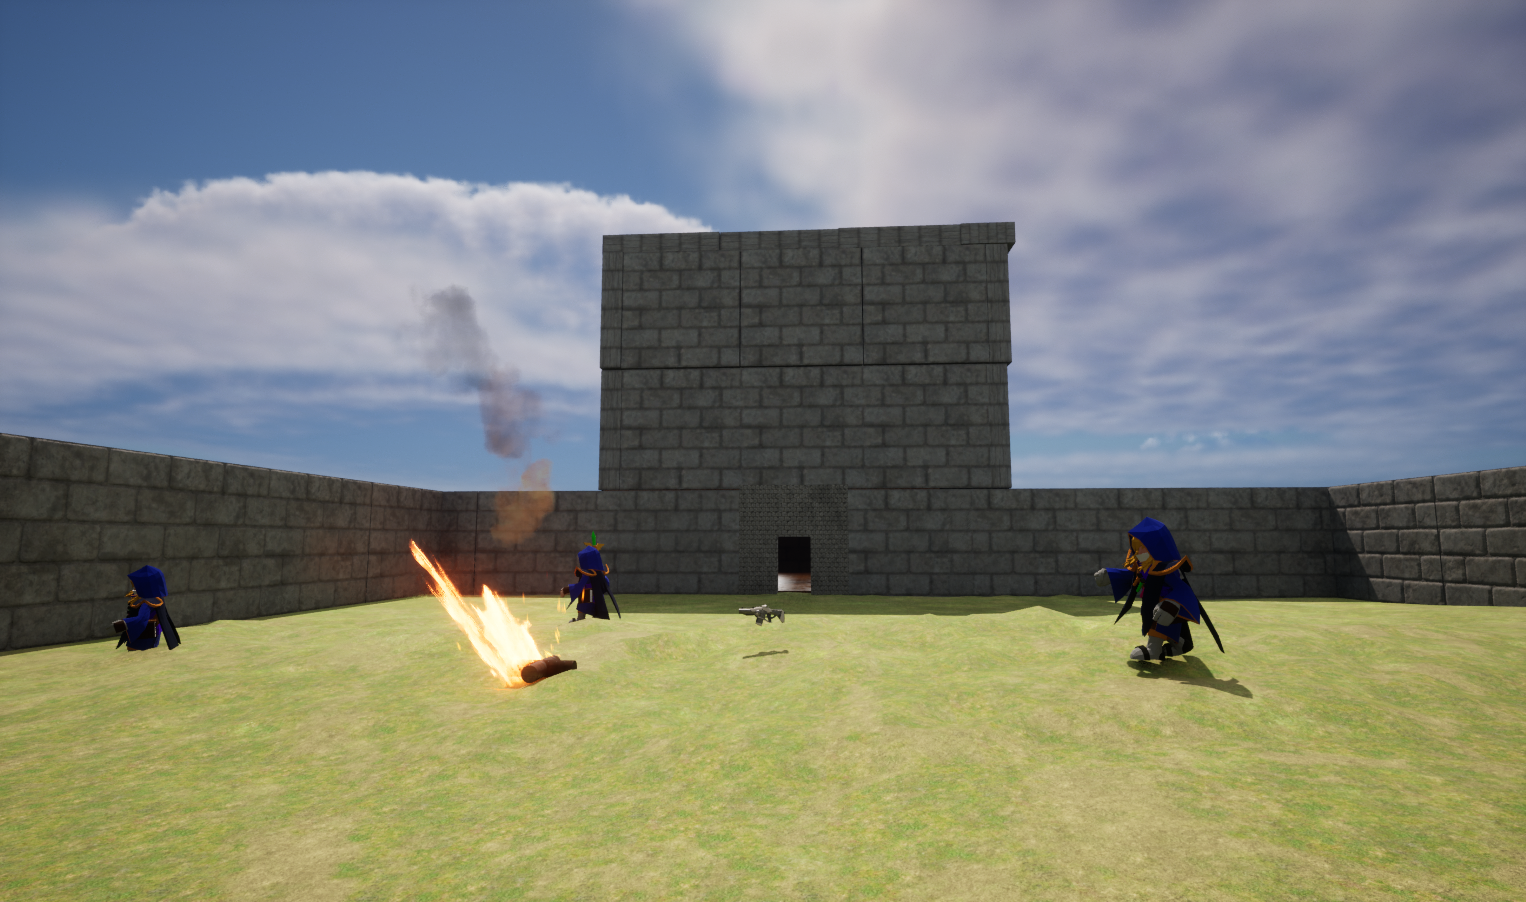
\includegraphics[width=10cm]{figures/unknown.png}
  \end{center}
}


\section{Sections--a useful organizational tool.}

\frameT{Summary}{
  \begin{enumerate}
    \item Any Questions or comments?
    \bigskip
    \item contact info
    \bigskip
    \item email:jesamars@ut.utm.edu or jamcblan@ut.utm.edu
    \end{enumerate}
}



\begin{frame}[fragile]
\frametitle{Family Tree Knowledge Base}
Facts:
\begin{verbatim}
Verbatim is a great way of enumerating code/algorithmic ideas.
\end{verbatim}
\end{frame}




\begin{frame}[fragile]
  \frametitle{Social Network Graph}
  \begin{figure}[ht]
    \begin{minipage}[b]{0.53\linewidth}
      \centering
      Minipages are a great way to
    \end{minipage}
    \hspace{0.5cm}
    \begin{minipage}[b]{0.4\linewidth}
      \centering
      Line up side-by-side content.

    \end{minipage}
  \end{figure}
  
\end{frame}


\frameT{Results} {
  Describe any results of your work here.

  \bigskip

  Things that worked?

  \bigskip

  Things that didn't work?
}

\frameT{Conclusions} {
  Some bullet points here to wrap things up.
}

\frameT{Any Questions?} {
  
  \begin{center}
    Questions?
  \end{center}
  \begin{center}
    Comments?
  \end{center}

  \bigskip

  Further project/author information:
  \begin{center}
    
\includegraphics[width=4cm]{figures/6AnLddq.png}
  \end{center}
}

%\frameF{fragile test} {
%}

%% \frameF{Prolog Family Tree} {
%% \begin{verbatim}
%% hello
%% \end{verbatim}



%% }

%Empty Page
%\frameT{Frame 1}{
%}  


\end{document}
